\section{Range of Forces and Amplitudes}
\subsection{Yukawa Potential}
Looking at the Schrödinger equation:
\begin{equation}
  H Ψ = E Ψ
\end{equation}
where the energy solution must satisfy $E^2 = m^2c^{4} + p^2c^2$.  The energy and momentum operators are given by:
\begin{equation}
    E = iℏ \frac{∂}{∂t} \quad , \quad \vec{p} = -iℏ \vec{∇}
\end{equation}
The solution should $ϕ$ be a static one, representing a radial potential:
\begin{equation}
  ∇^2ϕ(r) = \frac{m^2c^2}{ℏ^2} ϕ(r)
\end{equation}
As the factors have units of length squared, we can create a new variable $R = ℏ^2 / m^2c^2$. Guessing a solution on the form $ϕ(r) = u(r) / r$, we get the following solution not diverging for large $r$:
\begin{equation}
  \frac{∂^2 u(r)}{∂ r^2} = \frac{u(r)}{R^2} →  u(r) = ae^{-r / R} →  ϕ(r) = a \frac{e^{-r / R}}{r}
\end{equation}
This gives a potential $V$ as seen in \cref{eq: yukawa_potential}, with a potential vanishing for large distances. For complex structures we need to take into the internal structure as well. This assumes an interaction between a particle with charge $-g$, and another much heavier particle with charge $+g$.
\begin{equation}\label{eq: yukawa_potential}
  V(r) = -\frac{g^2}{4π} \frac{e^{-r / R}}{r}
\end{equation}

\subsection{Yukawa Amplitude}
Amplitude from the Bourne approximation:
\begin{equation}
  \mathcal{M} = ∫ V(\vec{r}) e^{i \vec{q} ⋅ \vec{r} / ℏ} d^3r  \quad , \quad  \vec{q} = \vec{p}_f - \vec{p}_i
\end{equation}
Solving this with the Yukawa potential, we get the following result:
\begin{equation}
  \vec{q} ⋅ \vec{r} = qr \cos θ \quad , \quad  \mathrm{d}^3r = r^2 \mathrm{d}r = \sin \mathrm{d}θ \mathrm{d}r \mathrm{d}ϕ
\end{equation}
This gives the following result in \cref{eq: yukawa_amplitude}, only valid when $\left|\vec{q}_i\right| = \left|\vec{q}_f\right|$ and energy is constant (elastic scattering):
\begin{equation}\label{eq: yukawa_amplitude}
  \mathcal{M}(q^2) = - \frac{g^2 ℏ^2}{q^2 + m^2c^2}
\end{equation}

To make this Lorentz invariant (as momentum is dependant on the frame of reference), we get the following result in \cref{eq: yukawa_amplitude_lorentz}, when $Q^2 ≪ m^2$
\begin{equation}
  Q^2 (\vec{q}_i - \vec{q}_f)^ - (E_f - E_i)^2 / c^2
\end{equation}
\begin{equation}\label{eq: yukawa_amplitude_lorentz}
  \mathcal{M}(Q^2) = - \frac{g^2 ℏ^2}{Q^2 + m^2c^2}
\end{equation}
If the range of the exchange is very small, then $Q^2$ is also very small, giving us the following approximation:
\begin{equation}
  \mathcal{M}(Q^2) = - \frac{g^2 ℏ^2}{m^2c^2} ≡ -G
\end{equation}
We often visualize this in Feynman diagrams as shown in \cref{fig: non_approx_exhange,fig: approx_exchange} . Both $Q^2$ and $G$ are Lorentz invariant. 
\begin{figure}[h!]
\centering
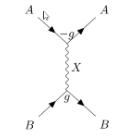
\includegraphics[width = .35\textwidth]{non_approx_exhange.png}
\caption{Feynman diagram of a non-approximated exchange of particle $X$}
\label{fig: non_approx_exhange}
\end{figure}

\begin{figure}[h!]
\centering
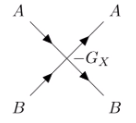
\includegraphics[width = .35\textwidth]{approx_exchange.png}
\caption{Feynman diagram of an short-range approximated exchange of particle $X$}
\label{fig: approx_exchange}
\end{figure}

\subsection{Amplitude of $W$-boson Exchange}
As the result of the short-range approximation shows in \cref{eq: yukawa_amplitude_lorentz}, we see it is dependant on mass, an therefore we can use this to calculate the mass of the $W$-boson. The amplitude of the $W$-boson exchange is given by:
\begin{equation}
  α_{W} ≡ \frac{g^2_{W}}{4πℏc}  \quad , \quad  α_{EM} = \frac{e^2}{4πϵ_0ℏc}
\end{equation}
Taking into account the spins of the particles gives a factor of $\sqrt{2}$. 
\begin{equation}
  G_{F} ? \frac{g^2_{W}ℏ^2}{m^2_{W}c^2}\sqrt{2} → \frac{G_{F}}{(ℏc)^3} = \frac{4πα_{W}}{(m_{Wc^2})^2} \sqrt{2}
\end{equation}
By measurement of $G_{F} / (ℏc)^3 = 1.166 ⋅  10^{-5}$ GeV$^{-2}$, we can calculate the mass of the $W$-boson to be $m_{W} ≈ 105$ GeV/c$^2$, which is close to the actual value of $m_{W} = 80.4$ GeV/c$^2$. This assumes $α_{W} ≈ α_{EM}$. 

\subsection{Amplitude of Other exchanges}
Each vertex has a factor charge and a cross section decay rate which is proportional to $\left|\mathcal{M}\right|^2$. We can count the number of exchanges of particle $X$ as orders of $α_{X}$ ($\sqrt{α_{X}}$, per vertex before squaring). This typically represent small corrections as $α_{X} ≪ 1$. 

\subsection{Muon vs Tau Decays}
\begin{equation}
  μ^- → e^- + \bar{ν}_e + ν_μ
\end{equation}
\begin{equation}
  τ^- → e^- + \bar{ν}_e + ν_τ
\end{equation}
The width of the decay rate is proportional to the matrix elements square: $Γ \propto \left|\mathcal{M}\right|^2$ and $\mathcal{M} \propto G_{F}, G_{f} = 1.166 ⋅  10^{-5} (ℏc)^3 /$GeV$^2$. To get units of energy we must have 
\begin{equation}
  Γ = K G^2_{F}(m_lc^2)^{5} / (ℏc)^{6}
\end{equation}
where $m_l$ is the mass of the initial lepton. We do not need to know $K$ as we only want to compare the two processes. In natural units we get:
\begin{equation}
  KG^2_{F} m_l^{5}
\end{equation}
The ratio then becomes as shown in \cref{eq: muon_tau_ratio}. As the muon only have one decay channel, it is easy to find the decay width. This does not hold for the tau, as it only becomes an electron about 18\% of the time.
\begin{equation}\label{eq: muon_tau_ratio}
  \frac{Γ(τ^{-} → e^{-} \bar{ν}_e ν_{τ})}{Γ(μ^{-} → e^{-} \bar{ν}_e ν_{μ})} ≈ \left(\frac{m_τ}{m_μ}\right)^{5} ≈ 1.354 ⋅  10^{6}
\end{equation}
We must correct for the fact that the tau decays into a muon about 17.8\% of the time, by using their respective lifetime $τ ≡ \frac{1}{Γ}$. Fort he muon we have $\frac{1}{τ_{μ}} = 1 / 2.2 μ$ seconds, and fore the tau we have $\frac{1}{τ_{τ}} = 1 / 0.29 p$ seconds. Using experiment telling us the branching fraction of the tau, we find we a good estimate of the ratio in \cref{eq: muon_tau_ratio}.
\begin{equation}
  \frac{Γ(τ^{-} → e^{-} \bar{ν}_e ν_{τ})}{Γ(μ^{-} → e^{-} \bar{ν}_e ν_{μ})} = \frac{τ_{μ}}{τ_{τ}} \underbrace{B(τ^{-} → e^{-} \bar{ν}_e ν_{τ})}_{17.8 \%} = 1.35 ⋅  10^{6} 
\end{equation}
which is very good estimate within $2\%$ of the predicted value. 


\section{Resonance Formation and Decay}
\begin{itemize}
  \item Cross-section is proportional to the following:
  \begin{equation}
    σ \propto χ^{*}(E) χ(E) \quad , \quad  χ(E) ∫_{0}^{∞} Ψ(t)e^{iωt} \ \mathrm{d}t  ω = E / ℏ
  \end{equation}
  \item The center of mass of the particle has 0 momentum. This gives:
  \begin{equation}
    Ψ(t) = Ψ(0) e^{-iω_{R}t} e^{- Γt / 2} \quad , \quad  ω_{R} = E_{r} / ℏ = m_{R}c^2 / ℏ
  \end{equation}
  \item The result is 
  \begin{equation}
    χ^{*}(E) χ(E) ∝ \frac{1}{(E - m_{R}c^2)^2 + ℏ^2 Γ^2 / 4}
  \end{equation}
  \item Visualized it looks like a Gaussian curve, but with a much higher peak. This is called a Breit-Wigner formula as shown in \cref{fig: breit-wigner_formula}. It tells us the width of the decay rate $Γ$ in energy units, and lets us look at decay rates of particles with very short lifetimes.
  \begin{figure}[h!]
  \centering
  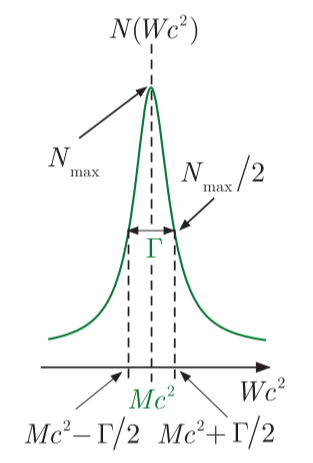
\includegraphics[width = .35\textwidth]{breit-wigner_formula.png}
  \caption{The Breit-Wigner formula for resonance formation and decay}
  \label{fig: breit-wigner_formula}
  \end{figure}
\end{itemize}
\subsubsection{Width and Lifetime}
\begin{itemize}
  \item In practical units: $λ ≡ Γ = 1 / τ$. 
  \item In natural units (energy in this case) : $Γ = ℏ / τ = ℏc / τc$
  \item The wider the width, the shorter the lifetime. 
\end{itemize}

\section{Neutrino Mixing and Oscillations}
\begin{itemize}
  \item Slowly, the neutrinos changes into each other. 
  \item The flavour eigenstates are not the same as their mass eigenstates. 
  \item The neutrinos propagate as mass eigenstates, but are produced and detected as flavour eigenstates of the weak interaction. 
\end{itemize}

\subsection{Neutrino Mixing}
\begin{itemize}
  \item This has an extremely low probability of happening, and has not been observed in the lab.
\end{itemize}
\subsubsection{3-generation mixing}
\begin{itemize}
  \item Easier to understand with 2 generations.
  \item If we produce a beam of $ν_e$ with momentum $p$, we can observe it later at some distance $x$. 
  \item As the neutrinos are produced as a mix of mass eigenstates, they will propagate slightly differently because of their mass difference. Some will turn into $ν_μ$, written as: $ν_e →  ⊗  → ν_{μ}$
\end{itemize}

\subsection{Probability of Mixing}
Starting with a beam of only $ν_e$ at $t = 0$. We can calculate the time dependent state. 
\begin{equation}
  \begin{pmatrix*}[r]
   \ket{ν_e} \\
   \ket{ν_{μ}} \\
  \end{pmatrix*} = 
  \begin{pmatrix*}[r]
   \cos θ & \sin θ \\
   -\sin θ & \cos θ \\
  \end{pmatrix*}
  \begin{pmatrix*}[r]
   \ket{ν_1} \\
   \ket{ν_{2}} \\
  \end{pmatrix*} \quad \text{and} \quad  
  \begin{pmatrix*}[r]
    \ket{ν_e} \\
    \ket{ν_{μ}} \\
   \end{pmatrix*} = 
   \begin{pmatrix*}[r]
    \cos θ & -\sin θ \\
    \sin θ & \cos θ \\
   \end{pmatrix*}
   \begin{pmatrix*}[r]
    \ket{ν_1} \\
    \ket{ν_{2}} \\
   \end{pmatrix*}
\end{equation}
\begin{equation}
  \ket{ν(t)} = a(t) \cos θ \ket{ν_1} + b(t) \sin θ \ket{ν_2} \quad , \quad  a(t) = \exp \left(-i E_1 t\right) \ , \ b(t) = \exp \left(-i E_2 t\right)
\end{equation}
As we can both detect $ν_e$ and $ν_{μ}$, we can calculate each probability, with a superposition of their wavefunctions instead of $ν_1$ and $ν_2$. 
\begin{equation}
  \ket{ν(t)} = a(t) \cos θ \left(\cos θ \ket{ν_e} - \sin θ \ket{ν_{μ}}\right) + b(t) \sin θ \left(\sin θ \ket{ν_e} + \cos θ \ket{ν_{μ}}\right)
\end{equation} 
\begin{equation}
  \ket{ν(t)} = \Big(a(t) \cos ^2 θ + b(t)\sin ^2 θ\Big)\ket{ν_e} + \Big(b(t) \sin θ \cos θ - a(t) \sin θ \cos θ\Big) \ket{ν_{μ}}
\end{equation}
Only if $a = b$ for all $t$, there will be no mixing. The normalization is defined as:
\begin{equation}
  \left|\bra{ν_e}\ket{ν_e}\right|^2 ≡ \left|\bra{ν_{μ}}\ket{ν_{μ}}\right|^2 ≡ 1
\end{equation}

The probability of finding the muon neutrino is given by:
\begin{equation}
  P(ν_{μ}) = \left|\bra{ν_{μ}}\ket{ν(t)}\right|^2 = \left|\frac{b(t) - a(t)}{2}\right|^2 \sin ^2 2θ \quad , \quad  \text{using } \sin 2θ = 2 \sin θ \cos θ
\end{equation}
\begin{equation}
  \left|b(t) - a(t)\right|^2 = b^{*}b + a^{*}a - (a^{*}b + b^{*}a) = 2 - \exp \left(i(E_2 - E_1)t\right) - \exp \left(-i(E_2 - E_1)t\right)
\end{equation}
Using the fact that $\exp ix + \exp -ix = 2 \cos x$ and $\sin ^2 x / 2 = (1 - \cos x) / 2$ we get:
\begin{equation}
  2 - 2 \cos \left(E_2 - E_1\right)t = 4 \sin ^2 \left(\frac{E_2 - E_1}{2}t\right)
\end{equation}
We finally get the probability:
\begin{equation}
\underline{\underline{ P(ν_{μ}) = \left|\bra{ν_{μ}}\ket{ν(t)}\right|^2 = \sin^2θ\sin^2 \left(\frac{(E_2 - E_1)t}{2}\right)}}
\end{equation}
As long as $θ$ is nonzero, or the energies are equal, we get a probability oscillating between 0 and 1.

\subsubsection{Conclusion}
\begin{itemize}
  \item As the masses of the neutrinos are very small in comparison to their momentum, we say the energy is the momentum. This gives a new difference in energy:
  \begin{equation}
    E_2 - E_1 = \frac{m_2^2 - m_1^2}{2E}
  \end{equation} 
  \item for small masses, $v ≈ c$, so the position $L(t) \approx ct$. 
  \item We define a new constant in natural units $L_0 ≡ 4E / (m_2^2 - m_1^2)$
  \item We have a final result of the probability of oscillation as:
  \begin{equation}
    P(ν_{μ}) = \sin^2 2θ \sin^2 \left(\frac{L}{L_0}\right)
  \end{equation}
  \item The scale of these oscillations are very large, and therefore very hard to detect. 
\end{itemize}